\subsection{Webfrontend}\label{subsec:subsection-four-one}

Wie in der Designanalyse beschrieben, konzentrierte sich das Collectiqo-Redesign auf zahlreiche visuelle Verbesserungen.
Dazu gehören eine moderne Farbpalette in harmonischen Lilatönen, ein klares, abgerundetes Design, eine optimierte Navigation und flüssigere Seitenübergänge.
Potenziale für weitere Optimierungen wurden ebenfalls identifiziert.

\begin{figure}[h]
    \centering
    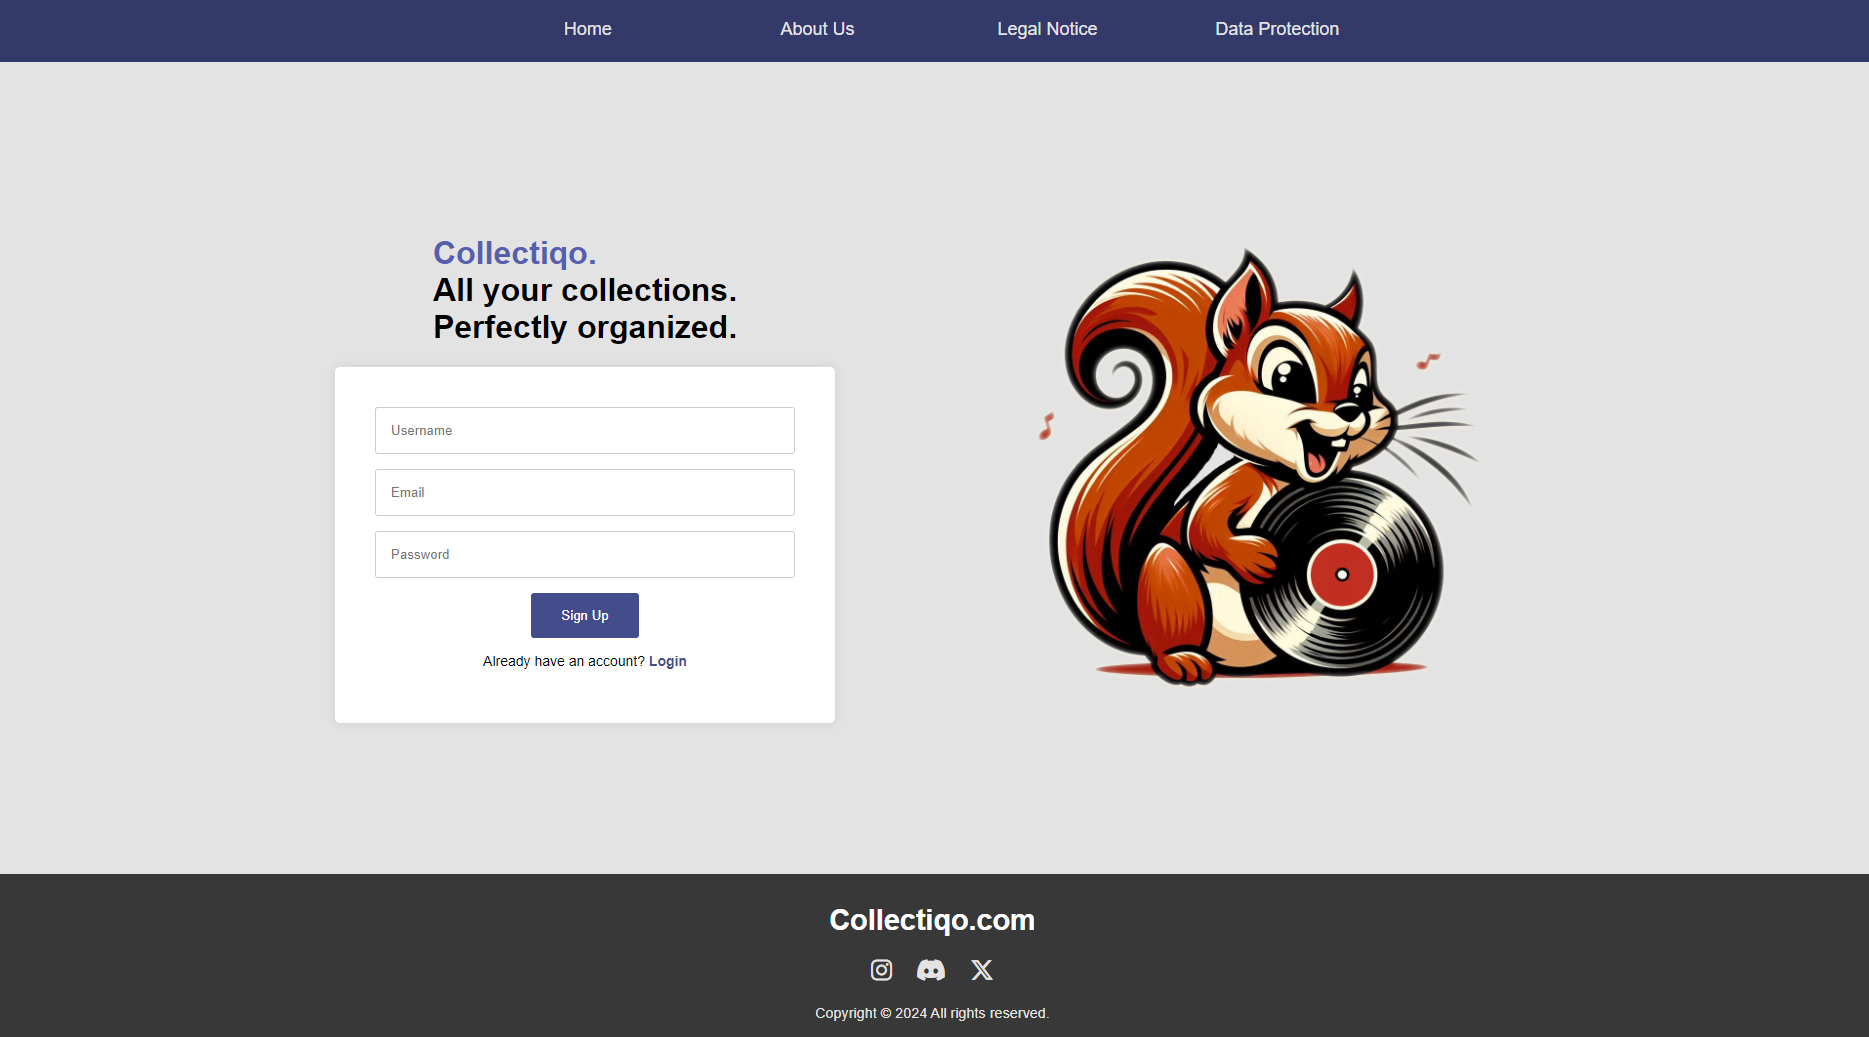
\includegraphics[width=0.9\textwidth]{landingHomePage}
    \caption{Landing Home Page}
    \label{fig:landingHomePage}
\end{figure}

Zu den besonders hervorstechenden Änderungen zählt ein neuer, charmanter Slogan, der zusammen mit dem Registrierungsfeld auf der linken Seite platziert wurde.
Das Maskottchen wurde entsprechend auf die rechte Seite verschoben, wodurch eine ausgewogene und einladende Gestaltung entsteht.
Die Lila Farbtöne lassen das Design modern wirken.

Der Header wurde um zusätzliche Navigationslinks erweitert, um die Benutzerführung zu verbessern:
\begin{itemize}
    \item \textbf{Home}: Verlinkt auf die Startseite.
    \item \textbf{About Us}: Führt zu einer Placeholder-Seite, die das Team vorstellt.
    \item \textbf{Legal Notice}: Enthält das Impressum des Teams.
    \item \textbf{Data Protection}: Erläutert die Datenschutzerklärung sowie den Umgang mit Benutzerdaten.
\end{itemize}

Der Footer enthält den Namen der Seite, Platzhalter-Icons für Social-Media-Verlinkungen sowie einen Copyright-Hinweis.

\begin{figure}[h]
    \centering
    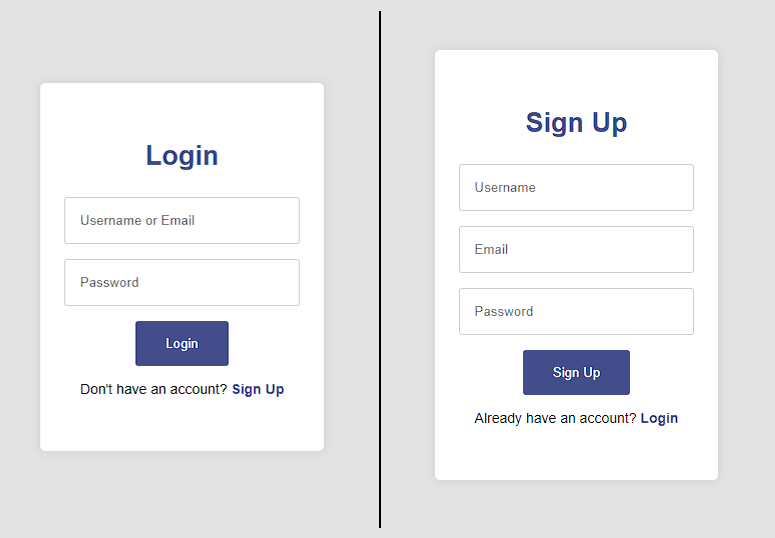
\includegraphics[width=0.5\textwidth]{loginSignUp}
    \caption{Login Sign-Up}
    \label{fig:loginSignUp}
\end{figure}

\pagebreak

Die separaten Login- und Sign-Up-Seiten wurden mit einem angepassten Hintergrund und einer Variation des Lilatons versehen.

Die allgemeine Struktur der persönlichen Benutzerseite blieb unverändert.
Auffällig ist jedoch die Einführung des neuen Lilatons, der das Design harmonisch abrundet.
Zusätzlich wurde der Hintergrund von Weiß auf ein sanftes Grau geändert, um die Darstellung augenfreundlicher zu gestalten.

\begin{figure}[h]
    \centering
    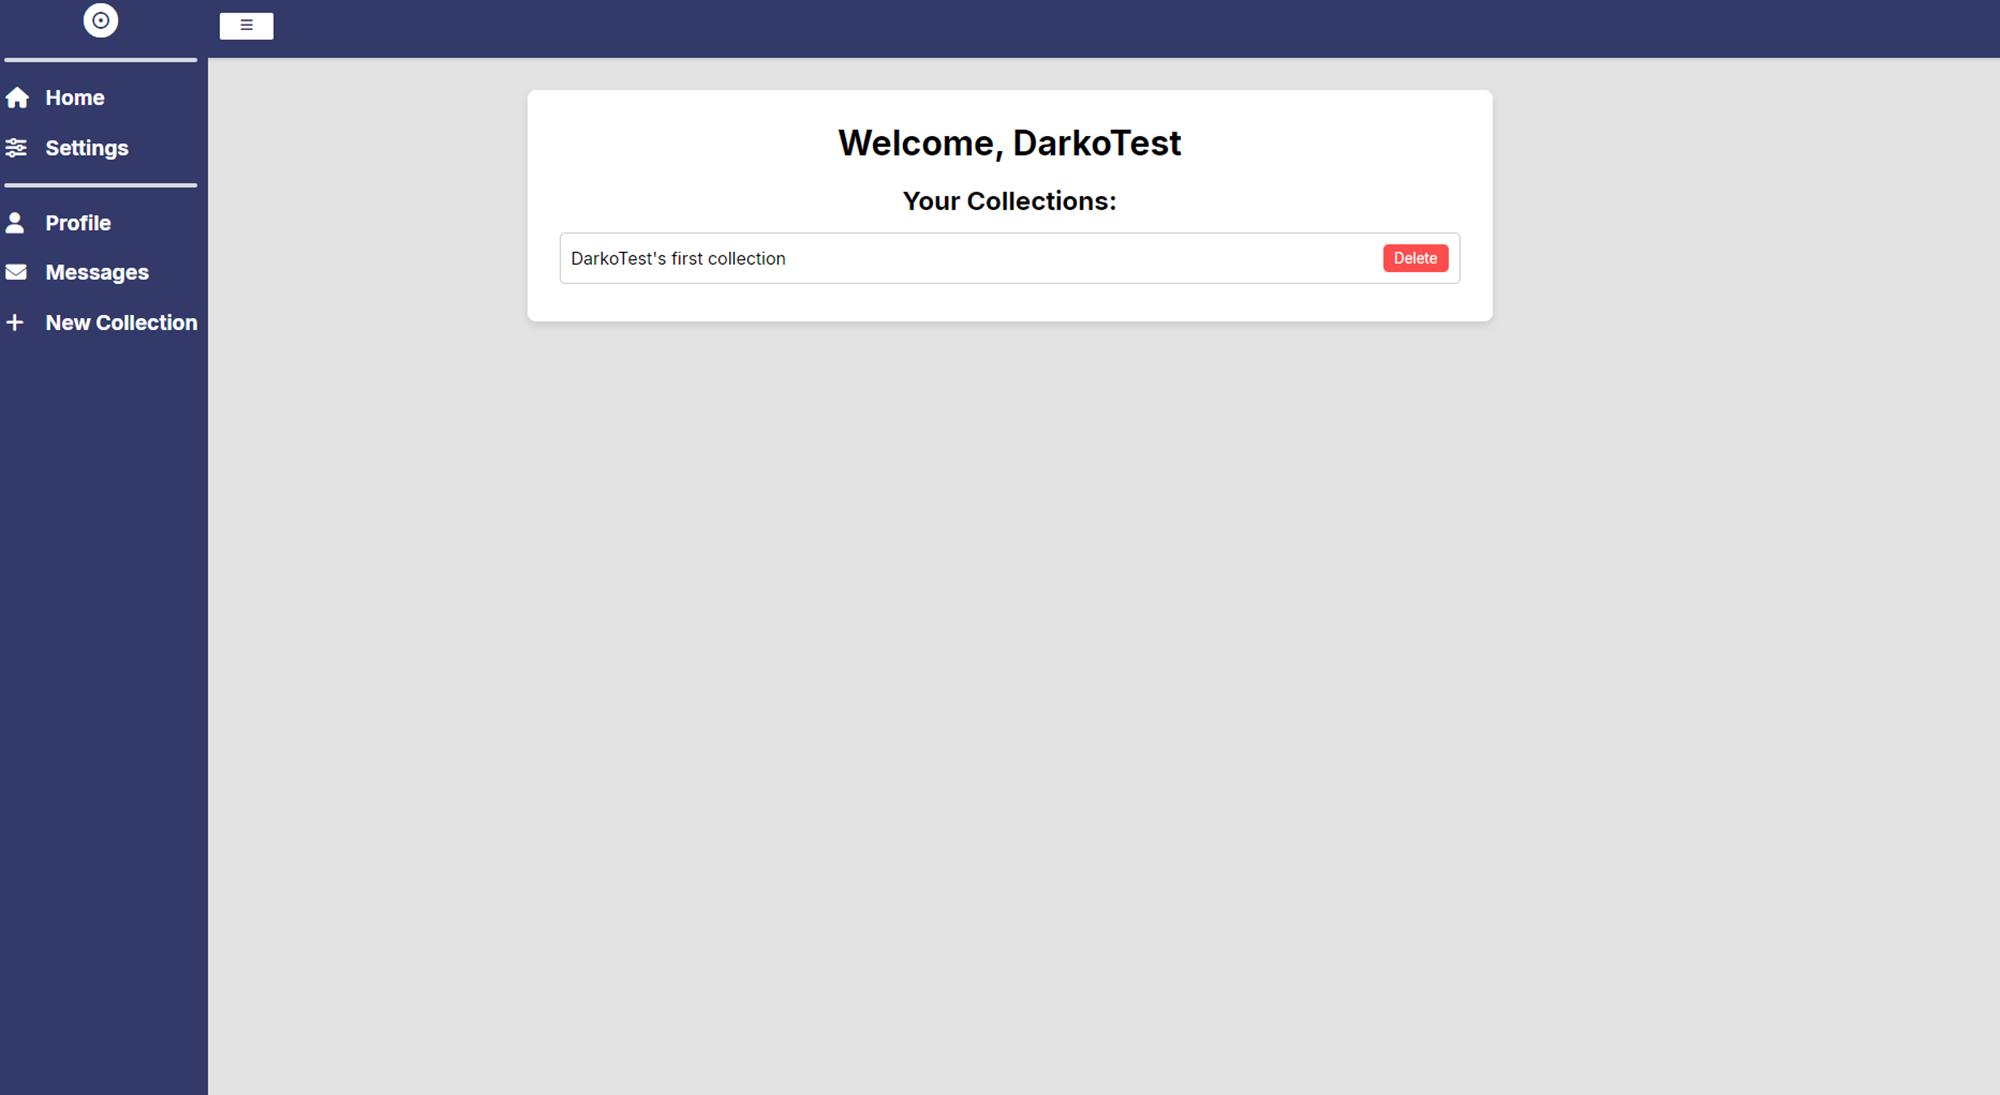
\includegraphics[width=1\textwidth]{userHome}
    \caption{User Home}
    \label{fig:userHome}
\end{figure}

\pagebreak

\begin{figure}[h]
    \centering
    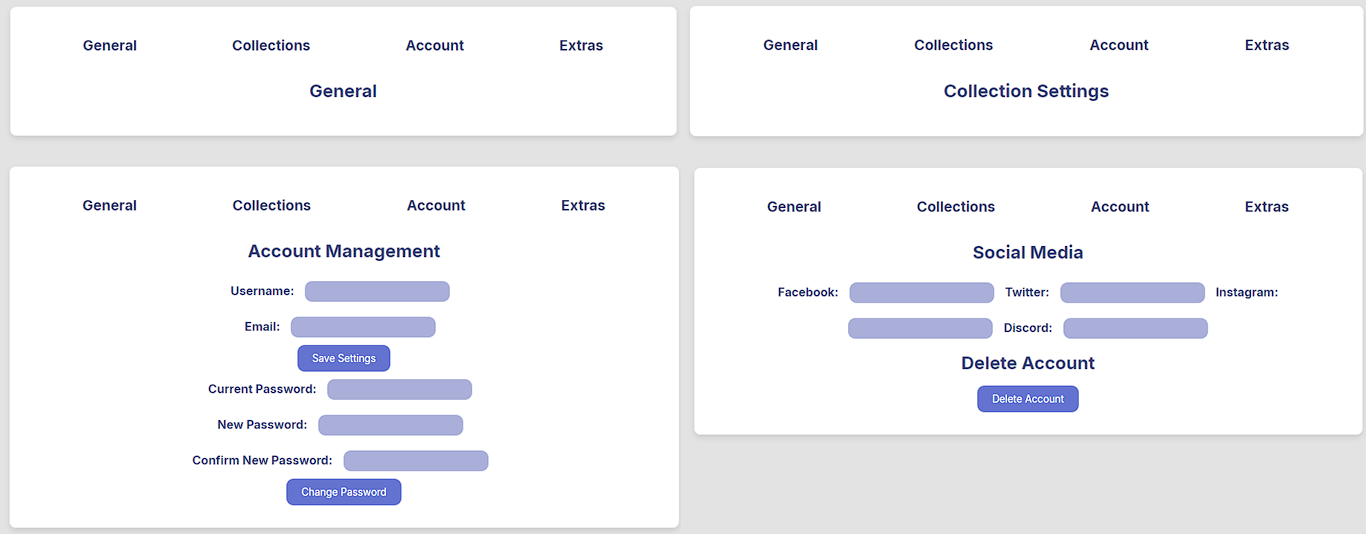
\includegraphics[width=0.9\textwidth]{accountSettings}
    \caption{Accounteinstellungen}
    \label{fig:accountSettings}
\end{figure}

Die Seite für Accounteinstellungen erhielt eine komplett neue Grundstruktur und wurde entsprechend den gleichen Designprinzipien überarbeitet.
Nutzer haben nun die Möglichkeit, ihre persönlichen Daten zu bearbeiten, ihren Namen anzupassen oder ihr Passwort zu ändern.

\begin{figure}[h]
    \centering
    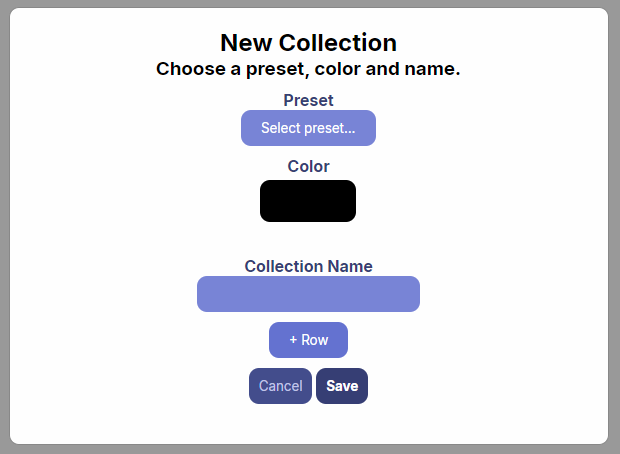
\includegraphics[width=0.6\textwidth]{addCollection}
    \caption{Collection Hinzufügen}
    \label{fig:addCollection}
\end{figure}

Das neue Fenster um eine Collection anzulegen wurde angepasst uns ist nun ansprechender für den Nutzer, was die zukünftige Bedienung erleichtern wird.
\pagebreak

\begin{figure}[h]
    \centering
    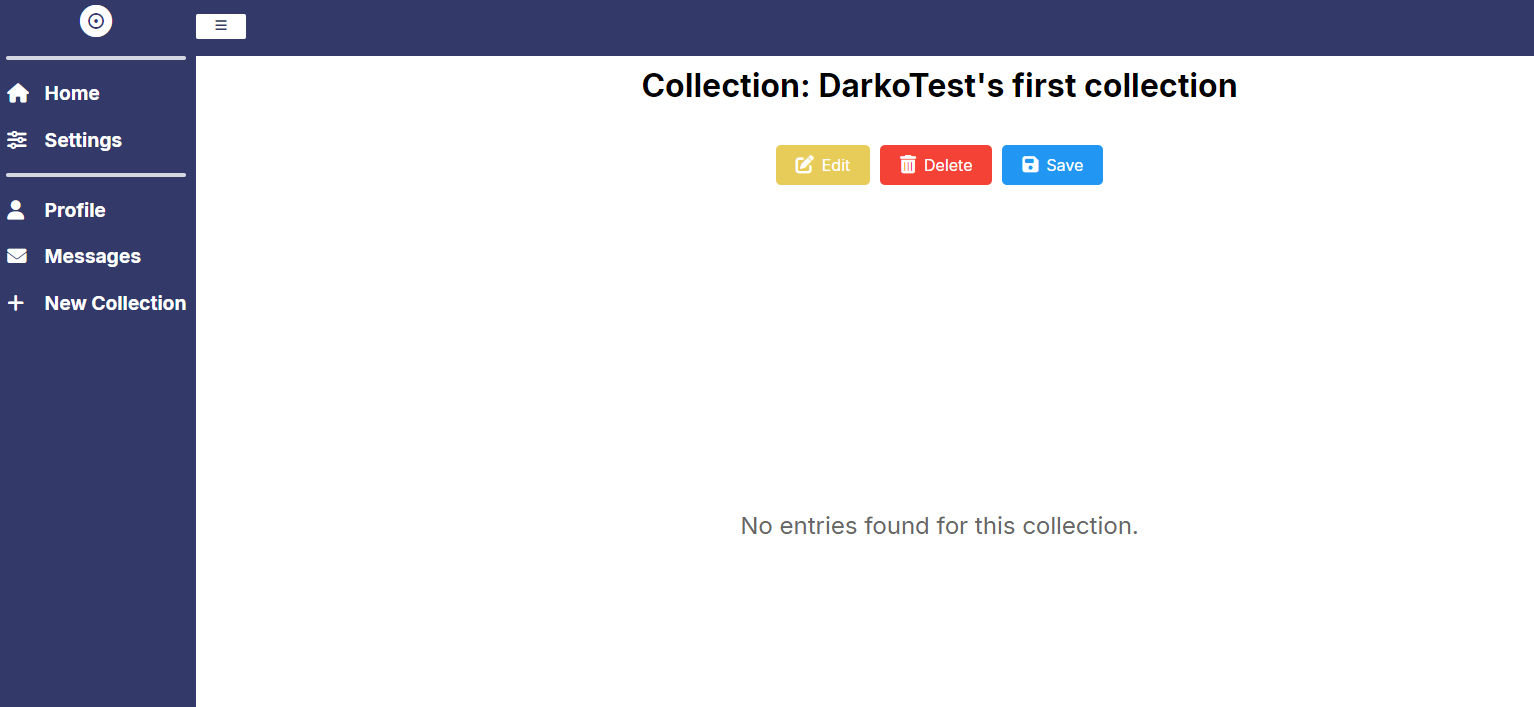
\includegraphics[width=0.9\textwidth]{collectionPage}
    \caption{Collection Ansicht}
    \label{fig:collectionPage}
\end{figure}

Abschließend wurde die Collection-Seite mit einer kleinen, aber wirkungsvollen Anpassung versehen.
Es sind nun drei farblich voneinander abgesetzte Knöpfe vorhanden, die eine schnelle und intuitive Anpassung der Collections ermöglichen.
Der \textbf{Speichern}-Knopf erscheint erst, nachdem der Nutzer die \textbf{Bearbeiten}-Funktion aktiviert hat, um eine übersichtliche und kontextsensitive Bedienung zu gewährleisten.
